\chapter{Adiabatic Quantum Computing}
\label{chap:aqc}

In this chapter we will explore the development of AQC as well as the physics of the adiabatic theorem.  We then discuss how adiabatic quantum computing works, and conduct a numerical simulation of an adiabatic quantum computation.

\section{A Brief History of AQC}
The idea of expanding simulated annealing to include quantum effects to solve problems was initially introduced by Kadowaki and Nishimori.\cite{transverse}  The linking of quantum annealing to quantum computation was done slightly later by Farhi et. al in 2000.\cite{farhi}  The structure of AQC appears here entirely intact: evolving from easily prepared initial Hamiltonians into problem Hamiltonians via the adiabatic theorem.  Farhi et. al.\cite{farhi} lacks any experimental or theoretical arguments for the speed of AQC, or comparison to gate model quantum computing.  Farhi et. al. followed up with another paper\cite{farhi2} with some preliminary simulations of AQC carried out by numerically integrating Schr\"odinger's Equation.  These results seemed to indicate exponential speedup over classical algorithms for an NP-Complete problem, but due to the difficulty of simulating quantum mechanics on a classical computer the maximum problem size they could experiment with was quite small so they could not draw very broad conclusions.

After this hopeful initial result it was shown by van Dam et. al.\cite{vandam} that, at least in principle, AQC is equivalent to gate model quantum computing.  Specifically they showed that adiabatic evolution taking time $T$ may be approximated by $O(T^2)$ unitary transformations of $n$ qubits.  However, van Dam et. al. also designed a class of minimization problems for which AQC has an exponential lower bound.  This was one of the earliest results in a controversy which continues to this day: how powerful are adiabatic quantum computers?  Proposed answers have included: being \emph{more} powerful than gate-model quantum computers, being able to solve NP-Complete problems efficiently;\cite{geordie}\cite{google} \emph{as} powerful as gate-model quantum computers;\cite{vandam} or no more powerful than classical computers.\cite{speedup}  Care must be taken to distinguish the questions of how powerful adiabatic quantum \emph{computing} is, and how powerful a \emph{given} adiabatic quantum computer is.

More papers on this topic followed, including several from A. P. Young with others.\cite{young3}\cite{young2}\cite{young1}  Using Quantum Monte Carlo techniques, they were able to increase the size of analyzable Hamiltonians from 24 spins to 256 spins.\cite{young1}
Their results seemed to indicate an exponential slowdown when solving a particular NP-Complete problem (Locked 1 in 3-SAT).\cite{young2}  This would suggest that an adiabatic quantum computer would \emph{not} be more powerful than a classical computer.

Concurrent with this effort to characterize adiabatic quantum computers theoretically was a commercial effort by D-Wave systems to build one.  Beginning with a single qubit\cite{qubit}, scaling to eight\cite{PhysRevB.82.024511} and then 128\cite{boixo2} and 512.\cite{pudenz}  While entanglement has been demonstrated to occur inside of this machine\cite{lanting}, the evidence for a quantum speedup is mixed,\cite{pudenz}\cite{boixo}\cite{smolin} with a very recent paper by R{\o}nnow et. al. suggesting that the \machine (the 512 spin machine) is not asymptotically faster than a classical computer.\cite{speedup}

In this work we carried out a variety of benchmarking on the \machine machine both to hopefully shed some light on the question of the speedup particular to this individual machine, and to validate our approach to problem compilation for AQC.

\section{The Adiabatic Theorem}

The central idea of Adiabatic Quantum Computation is solving problems by finding the ground states of specially constructed Hamiltonians.\cite{farhi}  Ground state relaxation is a form of analog computing where we rely on physics to do the calculating for us: we set up a physical system so that the ground state is the solution to our problem and let the system evolve.  Generally speaking, we expect that classical or quantum systems will still take exponentially long to reach this desired ground state for NP-hard problems.\cite{aaronson}
By starting the system in an easy to prepare state (for example, if your system was composed of spins then an easy to prepare state would be all spins ferromagnetically aligned) and then evolving adiabatically into our prepared problem state AQC uses the \emph{adiabatic theorem} to (hopefully) avoid this exponential delay.

The adiabatic theorem states that if a system is initially prepared in the ith energy level $\ket{\psi_i}$, and the Hamiltonian is evolved according to the adiabatic condition, the system will remain in the ith state after the evolution.  The adiabatic condition is:

\begin{equation}
	\left | \hbar\frac{\partial}{\partial t} \braket{\psi_f | \hat{V}(t) | \psi_i} \right | << \Delta^2
\end{equation}

where the energy gap between states $\ket{\psi_i}$ and $\ket{\psi_f}$ is $\Delta = |E_f - E_i|$ and $\hat{V}(t)$ is the time dependant part of the Hamiltonian.  For a derivation of the adiabatic theorem see Appendix \ref{apx:aqc}.  When the adiabatic condition is satisfied the probability of transition from state $i$ to state $f$ is zero, that is

\begin{equation}
	|\braket{\psi_f|\psi_i}|^2 \rightarrow 1
\end{equation}

So if the speed at which the Hamiltonian changes (the derivative term) is slow enough, and the gap $\Delta$ between the initial state and the other states is large enough, then the system won't transition into a new state.

\section{Finding a Problem Hamiltonian}
\label{sec:prob_ham}
While in principle there are an unlimited number of ways to construct a Hamiltonian whose ground state encodes the solution to a computation, our method is to use N 2-spin particles with a Hamiltonian:

\begin{equation}
	\label{eq:ham}
	\ham_f = \sum_i h_i \sigma_i^Z + \sum_{i < j} J_{ij} \sigma_i^Z\sigma_j^Z 
\end{equation}
where $\sigma_i^Z$ is the z-pauli matrix of the ith particle and $h_i$ and $J_{ij}$ are the parameters of the Hamiltonian; using spin as our computational basis we choose logical 1 (\texttt{true}) to be represented by spin up $\ket{\uparrow}$ (or $s = +1$) and logical 0 (\texttt{false}) by spin down $\ket{\downarrow}$ (or $s = -1$).  We call the $h_i$ parameters fields and the $J_{ij}$'s couplings.  The parameters $h_i$ control the tendency of the ith particle to point up or down, while the $J_{ij}$'s control the tendency of the ith and jth particles to align or anti-align.

We can find the energy of a state by multiplying each $h_i$ by the corresponding spin $s_i = \pm 1$ and each $J$ by the corresponding pair of spins $s_i$ and $s_j$.  Choosing a problem Hamiltonian is then the problem of finding the $h$s and $J$s so that the ground state corresponds to the problem we are trying to solve.  For example, we can encode the logic of a digital \texttt{NAND} gate using the collection of $h_i$'s and $J_{ij}$'s shown in Table \ref{tab:couplings} (the procedure for generating this Hamiltonian is described in Section \ref{sec:lin_prog}).  There are four degenerate ground states of this Hamiltonian, each corresponding to one of the entries in the logic table for a \texttt{NAND} gate.

\begin{table}
	\begin{center}
		\begin{tabular}{l l l}
			\begin{tabular}{r r | l}
				$A$ & $B$ & $C$ \\ \hline
				0 & 0 & 1 \\
				0 & 1 & 1 \\
				1 & 0 & 1 \\
				1 & 1 & 0 \\
			\end{tabular} &			
			\begin{tabular}{l | l}
				Fields & Couplings \\ \hline
				$h_A = -1$ & $J_{AB} = 1$ \\
				$h_B = -1$ & $J_{AC} = 2$ \\
				$h_C = -2$ & $J_{BC} = 2$ \\
			\end{tabular} &
			\begin{tabular}{r r r | l}
				$A$ & $B$ & $C$ & Energy \\ \hline
				$\downarrow$ & $\downarrow$ & $\downarrow$ & \ 9 \\
				$\downarrow$ & $\downarrow$ & $\uparrow$ & -3 \\
				$\downarrow$ & $\uparrow$ & $\downarrow$ & \ 1 \\
				$\downarrow$ & $\uparrow$ & $\uparrow$ & -3 \\
				$\uparrow$ & $\downarrow$ & $\downarrow$ & \ 1 \\
				$\uparrow$ & $\downarrow$ & $\uparrow$ & -3 \\
				$\uparrow$ & $\uparrow$ & $\downarrow$ & -3 \\
				$\uparrow$ & $\uparrow$ & $\uparrow$ & \ 1 \\
			\end{tabular}
		\end{tabular}
	\end{center}
	\caption[\texttt{NAND} Gate Fields and Couplings]{From left to right the truth table of the logical \texttt{NAND}; the fields and couplings that result in a Hamiltonian satisfying that truth table; the complete energy structure of that Hamiltonian.  Each state of the spins ($\uparrow/\downarrow$) whose logical equivalent appears in the truth table is part of the degenerate ground state of the final system.}
	\label{tab:couplings}
\end{table}


\begin{figure}
	\begin{center}
			\scalebox{0.5}{
				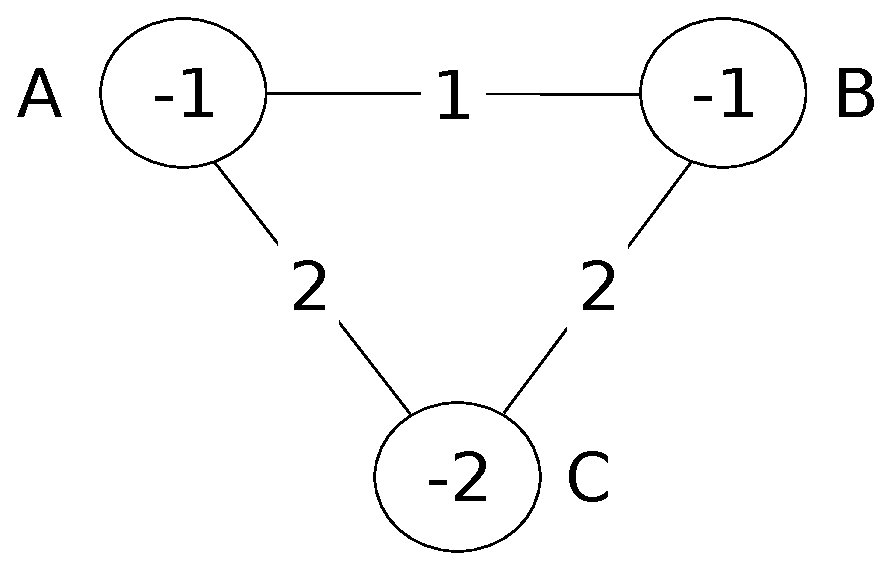
\includegraphics{img/nand.eps}
			} 
	\end{center}
	\caption[\texttt{NAND} Graph]{Graphical representation of the Hamiltonian implementing the logic of a \texttt{NAND} gate.  Each of the vertices is a spin and the number inside is the field value on that spin; each edge is the coupling value between the respective vertices.  Each ground state of this Hamiltonian enforces the logic $C = \neg(A \wedge B)$.}
	\label{fig:nand_graph}
\end{figure}



\section{Adiabatic Evolution}
Once we have a Hamiltonian whose ground state encodes the problem we would like to solve, we need to set up the evolution.  The Adiabatic Theorem lets us transition from the ground state of one Hamiltonian to another, so we need an initial Hamiltonian.  In general almost any Hamiltonian of which we know the ground state will work.  For simplicity we use the following initial Hamiltonian:
\begin{equation}
	\ham_i = \sum_i^N B \sigma_i^x
\end{equation}
where $B$ is some large constant.  This Hamiltonian has as it's ground state all the spins pointed along the (negative) x-axis (or equivalently, an equal superposition of $\ket{\pm z}$).  This is easy to prepare by applying a large magnetic field along the negative x direction.
Once we've assembled both our initial and final Hamiltonians, we can conduct the evolution.  We call the total Hamiltonian $H_{tot}$, and it is simply the sum of the initial and final Hamiltonian:

\begin{equation}
	\ham_{tot} = A(t)\ham_i + B(t)\ham_f
\end{equation}

where $A(t)$ and $B(t)$ are dimensionless functions of time such that $A(0) = B(T) = 1$ and $A(T) = B(0) = 0$ where $T$ is the final annealing time; this ensures that at $t = 0$ the Hamiltonian is equal to $H_i$ and at $t = T$ the Hamiltonian is equal to $H_f$.  Then the functions $A$ and $B$ describe the \emph{evolution path}.  Combining the evolution path with the speed at which the Hamiltonian is changing (or just the speed), that is $\frac{\partial A}{\partial t}$ and $\frac{\partial B}{\partial t}$, gives us the evolution trajectory.  

Given a ground state $\ket{psi_{gs}}$ of $\ham_{tot}$, the \emph{fidelity} ($\fid$) is the probability of measuring (after an anneal time $T$) $\psi_{gs}$, or $|\braket{\psi(T)|\psi_{gs}}|^2$.  If there are $N$ correct answer to our computation, and thus $\ket{\psi_N}$ degenerate ground states, the fidelity is defined as

\begin{equation}
	\fid = \sum_{i=0}^N \braket{\psi(T)|\psi_i}
\end{equation}

For a perfectly annealed system, the fidelity should go to one as the annealing time increases.  Since any real annealing will not be in the infinite anneal time limit, in practice our fidelity values are restricted to be $\leq 1$.  Hence AQC is fundamentally a probabilistic process.  The closer the fidelity is to 1, the more likely our computation is to succeed.  We will use the fidelity later in the experimental results section to evaluate how close we get to ideal AQC.

For a purely quantum mechanical system described by the Hamiltonian $\ham_{tot}$, the evolution trajectory completely determines the fidelity.
The simplest and most obvious trajectory is $A(t) = 1 - t/T$ and $B(t) = t/T$ at a constant speed, or a straight line path through Hamiltonian space.
There is no particular reason that a straight line from $(A=1,B=0)$ to $(A=0,B=1)$ should maximize the fidelity; indeed, because moving away from the origin in Hamiltonian space scales the Hamiltonian and its derived quantities up (including the energy gap), and the adiabatic condition is stated in terms of the energy gap, we expect that some more complicated curve through Hamiltonian space, potentially including changing the evolution speed, will give the best results.

However, in this work we restrict ourselves to evaluating straight line paths through Hamiltonian space due to the \machine being limited in this manner (see Chapter \ref{chap:machine}).

\section{Simulating AQC}
For small Hamiltonian we can simulate directly the process of quantum annealing by integrating the Schr\"odinger equation. For time dependent Hamiltonians such as ours, the general form of the Schr\"odinger equation is 

\begin{equation}
	i\hbar\frac{\partial}{\partial t} \ket{\psi(t)} = \ham\ket{\psi(t)}
	\label{eq:num_int}
\end{equation}

this is a system of linear ordinary differential equations which can be solved by numerical methods.  Using a fourth order Runge-Kutta method\cite{comp_book} we can find the overlap between the ground state $\ket{\psi_f}$ and the current state $\ket{\psi(t)}$ and plot this as a function of the annealing parameter.  We anneal an eight spin Hamiltonian (``k44\_and'', see Table \ref{tab:k44_and}) with linear control parameters $A(t) = 1-t/T$ and $B(t) = t/T$.  The state vector $\ket{\psi(t)}$ is written as a superposition over all the possible states
\begin{equation}
	\ket{\psi(t)} = \sum_{i=0}^{2^8-1} c_i(t)\ket{i}
\end{equation}

where $\ket{i}$ is a shorthand for 

\begin{align}
	\ket{0} &= \ket{\uparrow\uparrow\uparrow\uparrow\uparrow\uparrow\uparrow\uparrow}\notag\\
	\ket{1} &= \ket{\uparrow\uparrow\uparrow\uparrow\uparrow\uparrow\uparrow\downarrow}\notag\\
			& \vdots\notag\\
	\ket{255} &= \ket{\downarrow\downarrow\downarrow\downarrow\downarrow\downarrow\downarrow\downarrow}
\end{align}

where each $c_i(0) = 1/16$ (that is, an equal superposition) and we solve for all of the $c_i(t)$s using Equation \ref{eq:num_int} to generate each time step $c_i(t + \Delta t)$

Figure \ref{fig:simulate} shows the results of this simulation.  The features correspond to what we expect from the adiabatic theorem: the fidelity starts low and climbs as the system evolves.  It does not reach one as we are not in the adiabatic limit because we are annealing for only a finite time.  We expect to see similar results to the one shown here from experimental data; deviations will show us how far our experiments depart from the assumptions of AQC.
\begin{figure}
	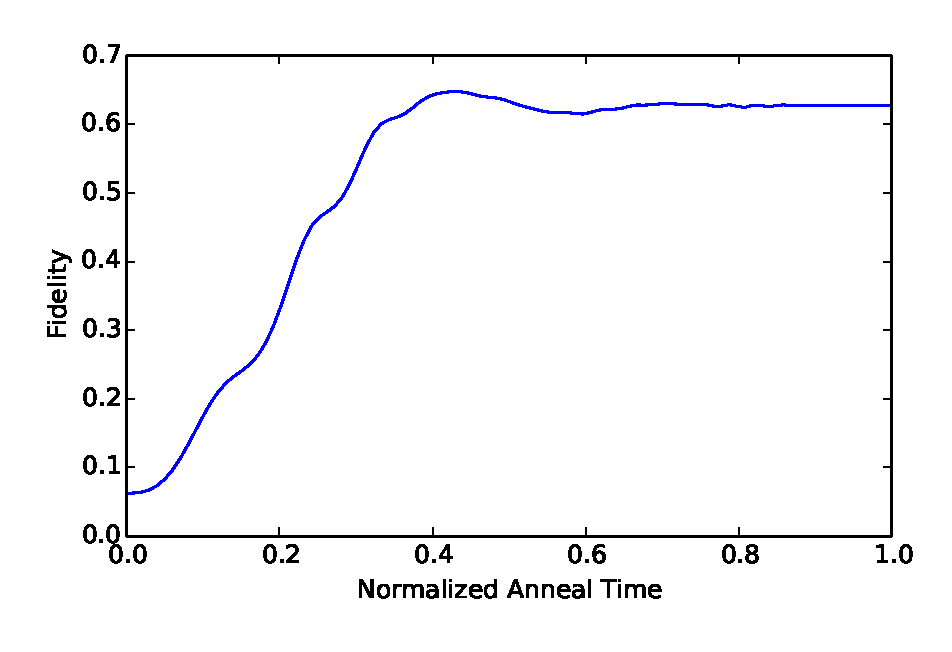
\includegraphics{img/simulate.eps}
	\caption[Simulated AQC]{Numerical simulation of adiabatic evolution by integrating the Schr\"odinger equation.}
	\label{fig:simulate}
\end{figure}
